\documentclass[
	ngerman,
	toc=listof, % Abbildungsverzeichnis sowie Tabellenverzeichnis in das Inhaltsverzeichnis aufnehmen
	toc=bibliography, % Literaturverzeichnis in das Inhaltsverzeichnis aufnehmen
	footnotes=multiple, % Trennen von direkt aufeinander folgenden Fußnoten
	parskip=half, % vertikalen Abstand zwischen Absätzen verwenden anstatt horizontale Einrückung von Folgeabsätzen
	numbers=noendperiod % Den letzten Punkt nach einer Nummerierung entfernen (nach DIN 5008)
]{scrartcl}
\pdfminorversion=5 % erlaubt das Einfügen von pdf-Dateien bis Version 1.7, ohne eine Fehlermeldung zu werfen (keine Garantie für fehlerfreies Einbetten!)

% Dokumenteninformationen ----------------------------------------------------
\newcommand{\titel}{User Manual}
\newcommand{\untertitel}{Studienarbeit \semester}
\newcommand{\kompletterTitel}{\titel{} \\ \untertitel}
\newcommand{\datum}{\today}

\newcommand{\vorlagenOrdner}{../99_Vorlagen} % Falls im Unterordner ../ vorne hinzufügen

\newcommand{\betriebLogo}{\vorlagenOrdner/Bilder/logo}

% Konfiguration -------------------------------------------------------------
\newcommand{\autoren}{
    \author{
        Schmid, Mike\\
        \texttt{sgschwin@hsr.ch}
        \and
        Schlatter, Janik\\
        \texttt{jschlatt@hsr.ch}
    }
}

\newcommand{\betreuer}{
    Stettler Beat\\
    \scriptsize \texttt{\url{beat.stettler@hsr.ch}}
    \normalsize
}

\newcommand{\schmid}{
    Mike Schmid\\
    \url{mschmid@hsr.ch}
    \normalsize
}

\newcommand{\schlatter}{
    Janik Schlatter\\
    \scriptsize \url{jschlatt@hsr.ch}
    \normalsize
}

\newcommand{\autorenNamen}{
    M. Schmid, J. Schlatter
}

\newcommand{\semester}{FS-2020}
\newcommand{\betriebName}{\textsc{HSR} Hochschule für Technik Rapperswil} % Metadaten zu diesem Dokument (Autor usw.)
% !TEX root = ../Projektdokumentation.tex

% Anpassung an Landessprache ---------------------------------------------------
\usepackage[english, main=ngerman]{babel} % \selectlanguage{english} if  needed

% Umlaute ----------------------------------------------------------------------
%   Umlaute/Sonderzeichen wie äüöß direkt im Quelltext verwenden (CodePage).
%   Erlaubt automatische Trennung von Worten mit Umlauten.
% ------------------------------------------------------------------------------
\usepackage[T1]{fontenc}
\usepackage[utf8]{inputenc}
\usepackage{textcomp} % Euro-Zeichen etc.

% Schrift ----------------------------------------------------------------------
\usepackage{lmodern} % bessere Fonts
\usepackage{relsize} % Schriftgröße relativ festlegen

% Tabellen ---------------------------------------------------------------------
\PassOptionsToPackage{table}{xcolor}
\usepackage{tabularx}
\usepackage{tabulary}
\usepackage{booktabs}
\usepackage{makecell}
\usepackage[table,xcdraw]{xcolor}
% für lange Tabellen
\usepackage{longtable}
\usepackage{array}
\usepackage{ragged2e}
\usepackage{lscape}
% Multi Columns
\usepackage{multicol}

% Grafiken ---------------------------------------------------------------------
\usepackage[dvips,final]{graphicx} % Einbinden von JPG-Grafiken ermöglichen
\usepackage{graphics} % keepaspectratio
\usepackage{floatflt} % zum Umfließen von Bildern
\graphicspath{{Bilder/}} % hier liegen die Bilder des Dokuments

% Sonstiges --------------------------------------------------------------------
\usepackage[titles]{tocloft} % Inhaltsverzeichnis DIN 5008 gerecht einrücken
\usepackage{enumitem} % anpassbare Enumerates/Itemizes
\usepackage{xspace} % sorgt dafür, dass Leerzeichen hinter parameterlosen Makros nicht als Makroendezeichen interpretiert werden

\usepackage{makeidx} % für Index-Ausgabe mit \printindex
\usepackage[printonlyused]{acronym} % es werden nur benutzte Definitionen aufgelistet

% Einfache Definition der Zeilenabstände und Seitenränder etc.
\usepackage{setspace}
\usepackage{geometry}

% Symbolverzeichnis
\usepackage[intoc]{nomencl}
\let\abbrev\nomenclature
\renewcommand{\nomname}{Abkürzungsverzeichnis}
\setlength{\nomlabelwidth}{.25\hsize}
\renewcommand{\nomlabel}[1]{#1 \dotfill}
\setlength{\nomitemsep}{-\parsep}

\usepackage{varioref} % Elegantere Verweise. „auf der nächsten Seite“
\usepackage{url} % URL verlinken, lange URLs umbrechen etc.

\usepackage{chngcntr} % fortlaufendes Durchnummerieren der Fußnoten
% \usepackage[perpage]{footmisc} % Alternative: Nummerierung der Fußnoten auf jeder Seite neu

\usepackage{ifthen} % bei der Definition eigener Befehle benötigt
\usepackage{todonotes} % definiert u.a. die Befehle \todo und \listoftodos
\usepackage[square]{natbib} % wichtig für korrekte Zitierweise

% PDF-Optionen -----------------------------------------------------------------
\usepackage{pdfpages}
\pdfminorversion=5 % erlaubt das Einfügen von pdf-Dateien bis Version 1.7, ohne eine Fehlermeldung zu werfen (keine Garantie für fehlerfreies Einbetten!)
\usepackage[
    bookmarks,
    bookmarksnumbered,
    bookmarksopen=true,
    bookmarksopenlevel=1,
    colorlinks=true,
% diese Farbdefinitionen zeichnen Links im PDF farblich aus
    linkcolor=AOBlau, % einfache interne Verknüpfungen
    anchorcolor=AOBlau,% Ankertext
    citecolor=AOBlau, % Verweise auf Literaturverzeichniseinträge im Text
    filecolor=AOBlau, % Verknüpfungen, die lokale Dateien öffnen
    menucolor=AOBlau, % Acrobat-Menüpunkte
    urlcolor=AOBlau,
% diese Farbdefinitionen sollten für den Druck verwendet werden (alles schwarz)
    %linkcolor=black, % einfache interne Verknüpfungen
    %anchorcolor=black, % Ankertext
    %citecolor=black, % Verweise auf Literaturverzeichniseinträge im Text
    %filecolor=black, % Verknüpfungen, die lokale Dateien öffnen
    %menucolor=black, % Acrobat-Menüpunkte
    %urlcolor=black,
%
    %backref, % Quellen werden zurück auf ihre Zitate verlinkt
    pdftex,
    plainpages=false, % zur korrekten Erstellung der Bookmarks
    pdfpagelabels=true, % zur korrekten Erstellung der Bookmarks
    hypertexnames=false, % zur korrekten Erstellung der Bookmarks
    linktocpage % Seitenzahlen anstatt Text im Inhaltsverzeichnis verlinken
]{hyperref}
% Befehle, die Umlaute ausgeben, führen zu Fehlern, wenn sie hyperref als Optionen übergeben werden
\hypersetup{
    pdftitle={\titel -- \untertitel},
    pdfauthor={\autoren},
    pdfcreator={\autoren},
    pdfsubject={\titel -- \untertitel},
    pdfkeywords={\titel -- \untertitel},
}


% zum Einbinden von Programmcode -----------------------------------------------
\usepackage{listings}
\usepackage{xcolor}
\usepackage{beramono}
% Pseudocode
\usepackage{algorithmic}
\usepackage[linesnumbered,ruled]{algorithm2e}

\definecolor{hellgelb}{rgb}{1,1,0.9}
\definecolor{colKeys}{rgb}{0,0,1}
\definecolor{colIdentifier}{rgb}{0,0,0}
\definecolor{colComments}{rgb}{0,0.5,0}
\definecolor{colString}{rgb}{1,0,0}
\definecolor{bluekeywords}{rgb}{0,0,1}
\definecolor{greencomments}{rgb}{0,0.5,0}
\definecolor{redstrings}{rgb}{0.64,0.08,0.08}
\definecolor{xmlcomments}{rgb}{0.5,0.5,0.5}
\definecolor{types}{rgb}{0.17,0.57,0.68}
\definecolor{DarkPurple}{rgb}{0.4, 0.1, 0.4}
\definecolor{DarkCyan}{rgb}{0.0, 0.5, 0.4}
\definecolor{LightLime}{rgb}{0.3, 0.5, 0.4}
\definecolor{Blue}{rgb}{0.0, 0.0, 1.0}
\definecolor{AOBlau}{rgb}{0, 0.28, 0.56}
% Tabellenfärbung:
\definecolor{heading}{rgb}{0.64,0.78,0.86}
\definecolor{odd}{rgb}{0.9,0.9,0.9}

\lstset{
    float=hbp,
	basicstyle=\footnotesize,
    identifierstyle=\color{colIdentifier},
    keywordstyle=\color{colKeys},
    stringstyle=\color{colString},
    commentstyle=\color{colComments},
    backgroundcolor=\color{hellgelb},
    columns=flexible,
    tabsize=2,
    frame=single,
    extendedchars=true,
    showspaces=false,
    showstringspaces=false,
    numbers=left,
    numberstyle=\tiny,
    breaklines=true,
    breakautoindent=true,
	captionpos=b,
}
\lstdefinestyle{visual-studio-style}{
	language=[Sharp]C,
	columns=flexible,
	showstringspaces=false,
	basicstyle=\footnotesize\ttfamily, 
	commentstyle=\color{greencomments},
	morekeywords={partial, var, value, get, set},
	keywordstyle=\bfseries\color{bluekeywords},
	stringstyle=\color{redstrings},
	breaklines=true,
	breakatwhitespace=true,
	tabsize=4,
	numbers=left,
	numberstyle=\tiny\color{black},
	frame=lines,
	showspaces=false,
	showtabs=false,
	escapeinside={£}{£},
}
\lstdefinestyle{eclipse-style}{
	language=Java,  
	columns=flexible,
	showstringspaces=false,     
	basicstyle=\footnotesize\ttfamily, 
	keywordstyle=\bfseries\color{DarkPurple},
	commentstyle=\color{LightLime},
	stringstyle=\color{Blue}, 
	escapeinside={£}{£}, % latex scope within code      
	breaklines=true,
	breakatwhitespace=true,
	showspaces=false,
	showtabs=false,
	tabsize=4,
	morekeywords={length},
	numbers=left,
	numberstyle=\tiny\color{black},
	frame=lines,
}
\lstset{style=eclipse-style}
\lstdefinelanguage{cs}{
	sensitive=false,
	morecomment=[l]{//},
	morecomment=[s]{/*}{*/},
	morestring=[b]",
	morekeywords={
		abstract,event,new,struct,as,explicit,null,switch
		base,extern,object,this,bool,false,operator,throw,
		break,finally,out,true,byte,fixed,override,try,
		case,float,params,typeof,catch,for,private,uint,
		char,foreach,protected,ulong,checked,goto,public,unchecked,
		class,if,readonly,unsafe,const,implicit,ref,ushort,
		continue,in,return,using,decimal,int,sbyte,virtual,
		default,interface,sealed,volatile,delegate,internal,short,void,
		do,is,sizeof,while,double,lock,stackalloc,
		else,long,static,enum,namespace,string},
}
\lstdefinelanguage{natural}{
	sensitive=false,
	morecomment=[l]{/*},
	morestring=[b]",
	morestring=[b]',
	alsodigit={-,*},
	morekeywords={
		DEFINE,DATA,LOCAL,END-DEFINE,WRITE,CALLNAT,PARAMETER,USING,
		IF,NOT,END-IF,ON,*ERROR-NR,ERROR,END-ERROR,ESCAPE,ROUTINE,
		PERFORM,SUBROUTINE,END-SUBROUTINE,CONST,END-FOR,END,FOR,RESIZE,
		ARRAY,TO,BY,VALUE,RESET,COMPRESS,INTO,EQ},
}
\lstdefinelanguage{php}{
	sensitive=false,
	morecomment=[l]{/*},
	morestring=[b]",
	morestring=[b]',
	alsodigit={-,*},
	morekeywords={
		abstract,and,array,as,break,case,catch,cfunction,class,clone,const,
		continue,declare,default,do,else,elseif,enddeclare,endfor,endforeach,
		endif,endswitch,endwhile,extends,final,for,foreach,function,global,
		goto,if,implements,interface,instanceof,namespace,new,old_function,or,
		private,protected,public,static,switch,throw,try,use,var,while,xor
		die,echo,empty,exit,eval,include,include_once,isset,list,require,
		require_once,return,print,unset},
}
 % verwendete Packages
% !TEX root = ../Projektdokumentation.tex

% Seitenränder -----------------------------------------------------------------
\setlength{\topskip}{\ht\strutbox} % behebt Warnung von geometry
\geometry{
	a4paper,
	left=20mm,
	right=20mm,
	top=25mm,
	bottom=40mm
}

\usepackage[
	automark, % Kapitelangaben in Kopfzeile automatisch erstellen
	headsepline, % Trennlinie unter Kopfzeile
	% footsepline, % Trennlinie oberhalb Fusszeile
	ilines % Trennlinie linksbündig ausrichten
]{scrpage2}

% Kopf- und Fußzeilen ----------------------------------------------------------
\pagestyle{scrheadings}
% chapterpagestyle gibt es nicht in scrartcl
%\renewcommand{\chapterpagestyle}{scrheadings}
\clearscrheadfoot

% Kopfzeile
\renewcommand{\headfont}{\normalfont} % Schriftform der Kopfzeile
\ihead{\large{\textsc{\titel}}\\ \small{\untertitel} \\[2ex] \textit{\headmark}}
\chead{}
%\ohead{\includegraphics[scale=0.125]{\betriebLogo}}
\setlength{\headheight}{20mm} % Höhe der Kopfzeile
%\setheadwidth[0pt]{textwithmarginpar} % Kopfzeile über den Text hinaus verbreitern (falls Logo den Text überdeckt)

% Fußzeile
\ifoot{\autorenNamen}
\cfoot{}
\ofoot{\pagemark}

% Überschriften nach DIN 5008 in einer Fluchtlinie
% ------------------------------------------------------------------------------

% Abstand zwischen Nummerierung und Überschrift definieren
% > Schön wäre hier die dynamische Berechnung des Abstandes in Abhängigkeit
% > der Verschachtelungstiefe des Inhaltsverzeichnisses
\newcommand{\headingSpace}{1.5cm}

% Abschnittsüberschriften im selben Stil wie beim Inhaltsverzeichnis einrücken
\renewcommand*{\othersectionlevelsformat}[3]{
  \makebox[\headingSpace][l]{#3\autodot}
}

% Für die Einrückung wird das Paket tocloft benötigt
%\cftsetindents{chapter}{0.0cm}{\headingSpace}
\cftsetindents{section}{0.0cm}{\headingSpace}
\cftsetindents{subsection}{0.0cm}{\headingSpace}
\cftsetindents{subsubsection}{0.0cm}{\headingSpace}
\cftsetindents{figure}{0.0cm}{\headingSpace}
\cftsetindents{table}{0.0cm}{\headingSpace}

% Allgemeines
% ------------------------------------------------------------------------------

\onehalfspacing % Zeilenabstand 1,5 Zeilen
\frenchspacing % erzeugt ein wenig mehr Platz hinter einem Punkt

% Schusterjungen und Hurenkinder vermeiden
\clubpenalty = 10000
\widowpenalty = 10000
\displaywidowpenalty = 10000

% Quellcode-Ausgabe formatieren
\lstset{numbers=left, numberstyle=\tiny, numbersep=5pt, breaklines=true}
\lstset{emph={square}, emphstyle=\color{red}, emph={[2]root,base}, emphstyle={[2]\color{blue}}}

\counterwithout{footnote}{section} % Fußnoten fortlaufend durchnummerieren
\setcounter{tocdepth}{\subsubsectionlevel} % im Inhaltsverzeichnis werden die Kapitel bis zum Level der subsubsection übernommen
\setcounter{secnumdepth}{\subsubsectionlevel} % Kapitel bis zum Level der subsubsection werden nummeriert

% Aufzählungen anpassen
\renewcommand{\labelenumi}{\arabic{enumi}.}
\renewcommand{\labelenumii}{\arabic{enumi}.\arabic{enumii}.}
\renewcommand{\labelenumiii}{\arabic{enumi}.\arabic{enumii}.\arabic{enumiii}}
 % Definitionen zum Aussehen der Seiten
% !TEX root = ../Projektdokumentation.tex

% Abkürzungen, ggfs. mit korrektem Leerraum
\newcommand{\bs}{$\backslash$\xspace}
\newcommand{\bspw}{bspw.\xspace}
\newcommand{\bzw}{bzw.\xspace}
\newcommand{\ca}{ca.\xspace}
\newcommand{\dahe}{\mbox{d.\,h.}\xspace}
\newcommand{\etc}{etc.\xspace}
\newcommand{\eur}[1]{\mbox{#1\,\texteuro}\xspace}
\newcommand{\evtl}{evtl.\xspace}
\newcommand{\ggfs}{ggfs.\xspace}
\newcommand{\Ggfs}{Ggfs.\xspace}
\newcommand{\gqq}[1]{\glqq{}#1\grqq{}}
\newcommand{\inkl}{inkl.\xspace}
\newcommand{\insb}{insb.\xspace}
\newcommand{\ua}{\mbox{u.\,a.}\xspace}
\newcommand{\usw}{usw.\xspace}
\newcommand{\Vgl}{Vgl.\xspace}
\newcommand{\zB}{\mbox{z.\,B.}\xspace}

% Befehle für häufig anfallende Aufgaben
\newcommand{\Abbildung}[1]{\autoref{fig:#1}}
\newcommand{\Anhang}[1]{\appendixname{}~\ref{#1}: \nameref{#1} \vpageref{#1}}
\newcommand{\includegraphicsKeepAspectRatio}[2]{\includegraphics[width=#2\textwidth,height=#2\textheight,keepaspectratio]{#1}}
\newcommand{\Zitat}[2][\empty]{\ifthenelse{\equal{#1}{\empty}}{\citep{#2}}{\citep[#1]{#2}}}
\newcommand{\Autor}[1]{\textsc{#1}} % zum Ausgeben von Autoren
\newcommand{\itemd}[2]{\item{\textbf{#1}}\\{#2}} % erzeugt ein Listenelement mit fetter Überschrift

% einfaches Wechseln der Schrift, z.B.: \changefont{cmss}{sbc}{n}
\newcommand{\changefont}[3]{\fontfamily{#1} \fontseries{#2} \fontshape{#3} \selectfont}

% Verwendung analog zu \includegraphics
\newlength{\myx} % Variable zum Speichern der Bildbreite
\newlength{\myy} % Variable zum Speichern der Bildhöhe
\newcommand\includegraphicstotab[2][\relax]{%
% Abspeichern der Bildabmessungen
\settowidth{\myx}{\includegraphics[{#1}]{#2}}%
\settoheight{\myy}{\includegraphics[{#1}]{#2}}%
% das eigentliche Einfügen
\parbox[c][1.1\myy][c]{\myx}{%
\includegraphics[{#1}]{#2}}%
}

% verschiedene Befehle um Wörter semantisch auszuzeichnen ----------------------
\newcommand{\Index}[2][\empty]{\ifthenelse{\equal{#1}{\empty}}{\index{#2}#2}{\index{#1}#2}}
\newcommand{\Fachbegriff}[2][\empty]{\ifthenelse{\equal{#1}{\empty}}{\textit{\Index{#2}}}{\textit{\Index[#1]{#2}}}}
\newcommand{\NeuerBegriff}[2][\empty]{\ifthenelse{\equal{#1}{\empty}}{\textbf{\Index{#2}}}{\textbf{\Index[#1]{#2}}}}

\newcommand{\Ausgabe}[1]{\texttt{#1}}
\newcommand{\Eingabe}[1]{\texttt{#1}}
\newcommand{\Code}[1]{\texttt{#1}}
\newcommand{\Datei}[1]{\texttt{#1}}

\newcommand{\Assembly}[1]{\textsf{#1}}
\newcommand{\Klasse}[1]{\textsf{#1}}
\newcommand{\Methode}[1]{\textsf{#1}}
\newcommand{\Attribut}[1]{\textsf{#1}}

\newcommand{\Datentyp}[1]{\textsf{#1}}
\newcommand{\XMLElement}[1]{\textsf{#1}}
\newcommand{\Webservice}[1]{\textsf{#1}}

\newcommand{\Refactoring}[1]{\Fachbegriff{#1}}
\newcommand{\CodeSmell}[1]{\Fachbegriff{#1}}
\newcommand{\Metrik}[1]{\Fachbegriff{#1}}
\newcommand{\DesignPattern}[1]{\Fachbegriff{#1}}

\newcommand{\muss}[1]{\textcolor{red}{#1}}
\newcommand{\soll}[1]{\textcolor{orange}{#1}}
\newcommand{\kann}[1]{\textcolor{blue}{#1}}

\newcommand{\success}[1]{\textcolor{greencomments}{#1}}
\newcommand{\fail}[1]{\textcolor{red}{#1}} % eigene allgemeine Befehle, die z.B. die Arbeit mit LaTeX erleichtern

\begin{document}

% Deckblatt ------------------------------------------------------------------
\phantomsection
\thispagestyle{plain}
\pdfbookmark[1]{Deckblatt}{deckblatt}
\begin{titlepage}
    \begin{center}
        \includegraphics[scale=1.5]{\betriebLogo}\\[10ex]

        \rule{\linewidth}{0.5mm}\\[2ex]
        {\huge \bfseries  \titel }\\[2ex]
        {\LARGE \untertitel }\\[2ex]
        {\large \datum}\\
        \rule{\linewidth}{0.5mm}\\[10ex]

        \begin{minipage}[t]{0.4\textwidth}
            \begin{flushleft} 
                \large \emph{Autoren:}\\
                    \large Mike \textsc{Schmid}\\
                    \scriptsize \texttt{mike.schmid@hsr.ch}\\[1ex]
                    \large Janik \textsc{Schlatter}\\
                    \scriptsize \texttt{janik.schlatter@hsr.ch}\\[1ex]
            \end{flushleft}
            \end{minipage}
            ~
            \begin{minipage}[t]{0.4\textwidth}
            \begin{flushright} 
                \large \emph{Supervisor:} \\
                Prof. Stettler \textsc{Beat}\\
                \scriptsize \texttt{beat.stettler@hsr.ch}\\[1ex]
            \end{flushright}
        \end{minipage}\\[40ex]

        \small
        \noindent
        Dieses Werk einschließlich seiner Teile ist \textbf{urheberrechtlich geschützt}.
        Jede Verwertung außerhalb der engen Grenzen des Urheberrechtgesetzes ist ohne
        Zustimmung des Autors unzulässig und strafbar. Das gilt insbesondere für
        Vervielfältigungen, Übersetzungen, Mikroverfilmungen sowie die Einspeicherung
        und Verarbeitung in elektronischen Systemen.

    \end{center}
\end{titlepage}
\cleardoublepage

% Preface --------------------------------------------------------------------
\pagenumbering{Roman}

% Inhaltsverzeichnis
\phantomsection
\pdfbookmark[1]{Inhaltsverzeichnis}{inhalt}
\tableofcontents
\cleardoublepage

\pagenumbering{arabic}
% Jede Überschrift 1 auf neuer Seite
\let\stdsection\section
\renewcommand\section{\clearpage\stdsection}

% Inhalt ---------------------------------------------------------------------
\section{Installation}
	\subsection{Installationsvoraussetzungen}
	NUTS2.0 sollte sich auf jedem Betriebssystem ausführen lassen.
	Für die Ausführung wird eine Python 3.7 installation (oder aktueller) benötigt.
	Diese kann unter https://www.python.org/downloads/ heruntergeladen werden.

	Um NUTS2.0 ausführen zu können, muss zuerst das Github-Repository geklont werden:\\
	https://github.com/EkoGuandor229/Network-Unit-Testing. 
	Danach können die verwendeten Module über das Requirements-File mit dem Befehl
	'pip install requirements.txt' installiert werden.

	\subsection{Ausführen}
	Das Programm kann zu testzwecken regulär in einer Programmierumgebung 
	wie zum Beispiel PyCharm ausgeführt werden.

	Um NUTS2.0 aus einer Konsole zu starten muss zum Root-Ordner NUTS2.0 navigiert werden. 
	Man kann das Programm mit dem Befehl: 'python -m nuts' starten. 
	Wenn man das GUI auslassen und direkt alle Tests ausführen möchte kann
	man mit dem Befehl: 'python -m nuts -r' starten.

	\subsubsection{Konfiguration}
	Im File 'Config.yaml' können die Pfäde aller Ordner geändert werden, um beispielsweise
	das Inventory oder die Resultate zentral in einem Repository zu verwalten. 
	Zusätzlich kann noch bestimmt werden, ob das GUI Per default übersprungen werden soll.

\section{Inventar}
	Um Netzwerktests auszuführen benötigt man zuerst ein Inventar mit Devices und 
	Device Connections.
	Die Devices sind die Netzwerkgeräte wie zum Beispiel Router oder Switches.
	Die Device Connections sind die Verbindungen zwischen den Devices.

	\subsection{Devices}
		Die Definitionen der Devices sind unter Resources/Inventory/Devices/Devices.yaml abgelegt:\\
		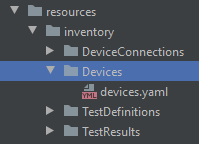
\includegraphics[scale=1.0]{\vorlagenOrdner/Bilder/Manual/Devices_yaml.png}

		Um neue Devices zu erfassen müssen folgende Informationen im yaml eingegeben werden:\\
		\begin{tabularx}{\textwidth}{lX}
			\toprule
			Attribut & Beschreibung \\
			\midrule
			device\_id & Eine eindeutige ID für das Device \\
			platform & Das OS welches das Device benutzt \\
			username & Der username welches das Device für das Login benutzt\\
			password & Das Passwort welches das Device für das Login benutzt\\
			hostname & Die Ip Adresse über welche das Device angesprochen werden kann\\
			loopback-addresse & IP-Addresse des Loopback-Interface. Für einige Tests benötigt.\\
			\midrule
		\end{tabularx}

		Diese Informationen sollten gemäss folgendem Beispiel dargestellt werden: \\
		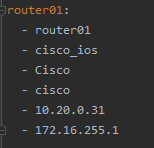
\includegraphics[scale=1.0]{\vorlagenOrdner/Bilder/Manual/Devices.png}

	\subsection{Device Connections}
		Die Definitionen der Device Connections sind unter \\
		Resources/Inventory/DeviceConnections/DeviceConnections.yaml abgelegt

		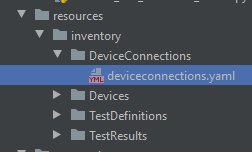
\includegraphics[scale=0.8]{\vorlagenOrdner/Bilder/Manual/DeviceConnections_yaml.png}

		Um Device Connections zu erfassen müssen folgende Informationen im yaml eingegeben werden:

		\begin{tabularx}{\textwidth}{ll}
			\toprule
			Attribut & Beschreibung \\
			\midrule
			device a & Die ID des ersten Devices \\
			device b & Die ID des zweiten Devices \\
			connection speed & Die Übertragungsrate der Verbindung\\
			\midrule
		\end{tabularx}

		Diese Informationen sollten wie folgt dargestellt werden: 

		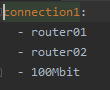
\includegraphics[scale=1.0]{\vorlagenOrdner/Bilder/Manual/DeviceConnections.png}

\section{Netzwerktests}
	Die Netzwerktests sind die Tests, welche effektiv auf dem zu testenden Netzwerk 
	ausgeführt werden sollen.
	Die Testdefinitionen befinden sich unter Resources/Inventory/TestDefinitions:

	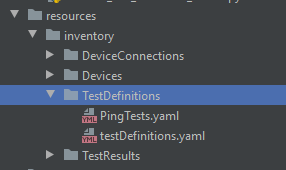
\includegraphics[scale=1.0]{\vorlagenOrdner/Bilder/Manual/TestDefinitions_yaml.png}

	Es können in diesem Ordner beliebig viele YAML Files abgelegt werden und es werden vonn allen Files die Tests erfasst.

	Um die Tests zu erfassen müssen folgende Informationen im yaml eingegeben werden:

	\begin{tabularx}{\textwidth}{ll}
		\toprule
		Attribut & Beschreibung \\
		\midrule
		test\_id & Eine eindeutige ID für den Test \\
		command & Ein Command um den Test zu bestimmen \\
		test\_device & Die ID des Devices auf welchem der Test ausgeführt werden soll\\
		target & Das Ziel (Zum Beispiel eine IP im Falle eines Pings)\\
		expected\_result & Das erwartete Resultat (Zum Beispiel Success im Falle eines Pings)\\
		test\_group & Ein Gruppenname um später die Tests zu Kategorisieren\\
		\midrule
	\end{tabularx}

	Diese Informationen sollten wie folgt dargestellt werden: 

	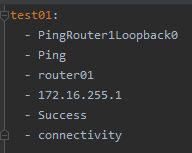
\includegraphics[scale=1.0]{\vorlagenOrdner/Bilder/Manual/TestDefinitions.png}
	\newpage

	\subsection{Commands}
		Folgende Commands sind bereits implementiert und können mit den jeweiligen expected\_results verwendet werden:
		\subsubsection{Ping}
			Führt einen Ping-Test auf das spezifizierte Target mit 4 ICMP Packeten aus.
			In der jetzigen Konfiguration wird eine 100\% Erfolgsquote erwartet, 
			damit der Ping-Test als erfolgreich gilt.
			Wenn andere Werte erwartet werden, muss dafür ein neuer Ping-Test implementiert
			werden, welche unterschiedliche Erwartungswerte implementiert hat.

			Als erwartetes Resultat kann 'Success' oder 'Failure' verwendet werden.

		\subsubsection{Show Interfaces}
			Der 'Show Interfaces'-Befehl benötigt kein Target, da die Interfaces des test\_device
			abgefragt werden. 
			Bei der Definition kann somit einfach 'No Target' eingegeben werden.
			Als erwartetes Resultat wird ein Dictionary mit key:'Interfacename' und 
			value:'True' oder 'False' verwendet werden.
			Dies sollte in folgender Form dargestellt werden:

			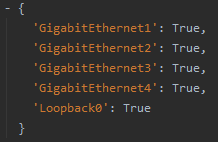
\includegraphics[scale=1.0]{\vorlagenOrdner/Bilder/Manual/ShowInterfaces.png}

		\subsubsection{Traceroute}
			Führt einen Traceroute vom test\_device auf das in target angegebene Ziel aus.
			Als erwartetes Resultat wird ein Array von IP Adressen angegeben.
			Diese müssen in der Reihenfolge, in denen die Hops im Traceroute besucht werden,
			angegeben werden. Für Hops, die keine IP-Addresse anzeigen, kann ein '*' in das
			Array eingetragen werden.

			Das Array bei expected\_result kann beispielsweise so aussehen:

			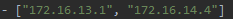
\includegraphics[scale=1.0]{\vorlagenOrdner/Bilder/Manual/Traceroute.png}

		\subsubsection{Arp Table}
			Für den Befehl 'Arp Table' wird kein Target benötigt, 
			da der Arp Table des im test\_device angegebenen Netzwerkgeräts abgefragt wird. 
			Es kann 'No Target' im 'target'-Feld eingegeben werden.
			Als erwartetes Resultat wird ein Array von Dictionaries erwartet. 
			In den Dictionaries werden folgende Informationen erwartet:

			\begin{tabularx}{\textwidth}{lX}
				\toprule
				Parametername & Parameterwert \\
				\midrule
				'interface': &  Name des Interface. \\
				'mac': &  MAC-Addresse des Nachbargeräts \\
				'ip': & IP-Addresse des Nachbargeräts \\
				\bottomrule
			\end{tabularx}

			Im Bild ist ein Beispiel des Arrays mit den Dictionaries in jeder Zeile angegeben:

			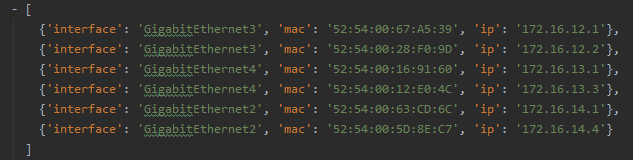
\includegraphics[scale=0.8]{\vorlagenOrdner/Bilder/Manual/ArpTable.png}

		\subsubsection{Ospf Neighbor}
			Für den Befehl 'Ospf Neighbor' wird kein Target benötigt, 
			da OSPF Nachbarn des im test\_device angegebenen Netzwerkgeräts abgefragt wird. 
			Es kann 'No Target' im 'target'-Feld eingegeben werden.	
			Als erwartetes Resultat wird ein Array mit Dictionaries erwartet. 
			In den Dictionaries werden folgende Informationen benötigt:

			\begin{tabularx}{\textwidth}{lX}
				\toprule
				Parametername & Parameterwert\\
				\midrule 
				'Neighbor-ID': & IP-Addresse des Nachbargeräts \\
				'Priority': & OSPF-Priorität als Ganzzahl\\
				'State': & Status des Nachbargeräts \\
				'Address': & IP-Addresse des Interface, über welches der Nachbar erreichbar ist. \\
				'Interface': & Name des Interface, über welches der Nachbar erreichbar ist. \\
				\bottomrule
			\end{tabularx}
			
			Das folgende Beispiel zeigt das Array von Dictionaries, wie es im YAML dargestellt wird:

			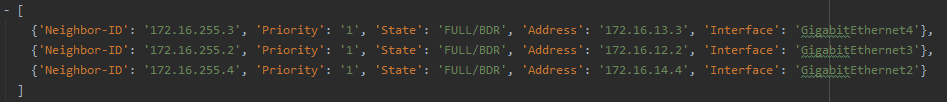
\includegraphics[scale=0.7]{\vorlagenOrdner/Bilder/Manual/OspfNeighbor.png}

\section{Durchführung}
	Nachdem dass Inventar erstellt und die Testdefinitionen erfasst wurden,
	kann man das Programm starten.
	Falls die Option Skip-GUI aktiviert wurde, werden alle Tests in der Reihenfolge durchgeführt,
	in der sie in der Testdefinition angegeben wurden. 
	Falls dies nicht aktiviert wurde öffnet sich ein Grafikinterface.

	\subsection{GUI}
		Das GUI für die Definition der Test Reihenfolge besteht aus zweit Tabs:

		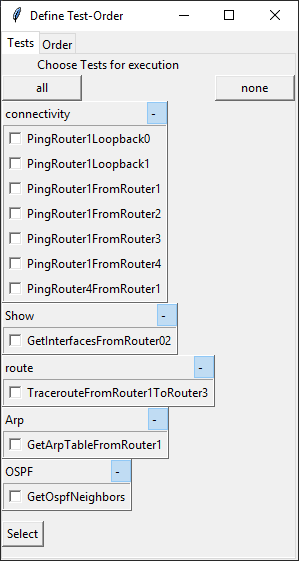
\includegraphics[scale=0.8]{\vorlagenOrdner/Bilder/Manual/GUI1.png}

		Im ersten Tab werden alle Tests nach Gruppen sortiert angezeigt.
		Die Gruppierung ist diejenige, die in der Testdefinition angegeben wurde. 
		Hier kann der Benutzer auswählen welche Tests er ausführen möchte.
		Nachdem die Tests ausgewählt wurden weden mit dem Button 'Select' 
		alle ausgewählten Tests selektiert und man kann danach die Reihenfolge der
		selektierten Test im zweiten Tab einstellen.

		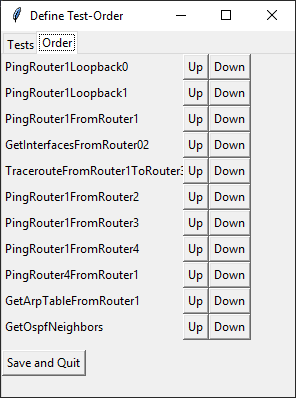
\includegraphics[scale=0.8]{\vorlagenOrdner/Bilder/Manual/GUI2.png}

		Im zweiten Tab werden alle selektierten Tests angezeigt und der Benutzer 
		kann mit den jeweiligen Buttons die Reihenfolge bestimmen.
		Nachdem der Benutzer mit der Reihenfolge zufrieden ist,
		kann mit dem Button 'Save and Quit' das GUI beendet werden.
		Alle selektierten Tests werden nun in der angegebenen Reihenfolge durchgeführt.

	\subsection{Test Resultate}
		Die Resultate der jeweiligen Durchführungen werden in der Konsole angezeigt 
		und zusätzlich noch in einem File gespeichert.
		Bestandene Tests werden nur mit ihrem Namen und dem Vermerk, dass der Test bestanden ist,
		angegeben. 
		Nicht bestandene Tests haben den Testnamen, das erwartete Ergebniss und das tatsächliche
		Ergebniss für einen soll-ist-Vergleich.

		Das folgende Bild zeigt eine komplette Durchführung des Programms mit elf bestandenen
		Tests und null nicht bestandenen Tests: 

		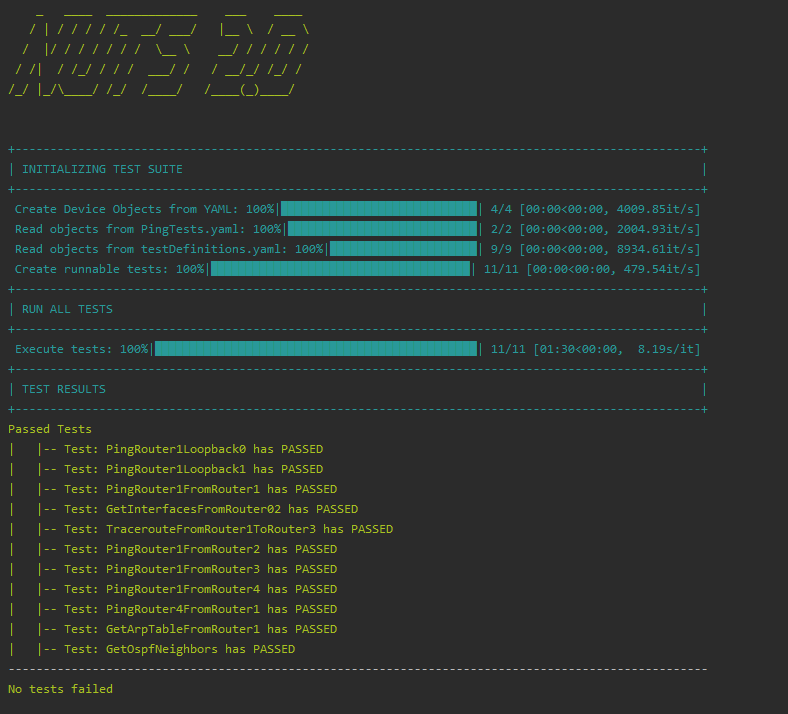
\includegraphics[scale=0.8]{\vorlagenOrdner/Bilder/Manual/ConsoleGUI.png}

		\newpage

		Das File, in dem der Testreport abgespeichert wird, befindet sich unter: 
		'Resources/Inventory/TestResults/results.txt'.

		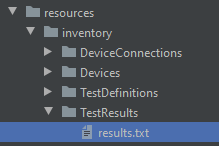
\includegraphics[scale=1.0]{\vorlagenOrdner/Bilder/Manual/TestResults_txt.png}

		In dem File wird zuerst der Zeitstempel der Testdurchführung angegeben, 
		danach werden zuerst die bestandenen Tests und am Schluss die nicht bestandenen Tests angezeigt.
		Bei den nicht bestandenen Tests werden zusätzlich noch das erwartete und das tatsächliche
		Resultat angezeigt.

		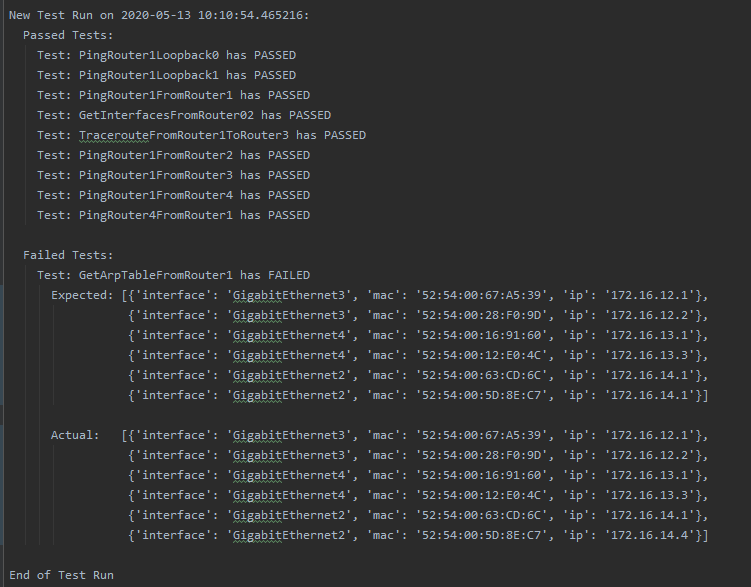
\includegraphics[scale=0.8]{\vorlagenOrdner/Bilder/Manual/TestResults.png}

\section{Neue Tests hinzufügen}
	Falls der Benutzer eigene Tests hinzufügen möchte,
	 müssen an folgenden Orten änderungen vorgenommen werden:

	\subsection{Conctrete Tests}
		Die konkreten Tests befinden sich unter 'nuts/testcreation/concretetests'
		In diesem Ordner muss ein neues Python-File angelegt werden.
		Im File wird der Test als Klasse implementiert.
		Es ist darauf zu achten, dass das Basisinterface 'NetworkTestStrategyInterface' 
		von der Testklasse implementiert wird, um davon die grundlegenden Funktionalitäten
		zu erben.

		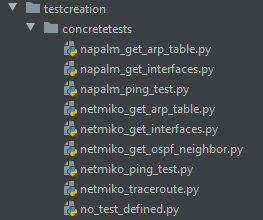
\includegraphics[scale=1.0]{\vorlagenOrdner/Bilder/Manual/concretetests.png}

		Nach der Erstellung muss der Test geschrieben werden.
		Dazu wird in der \_\_init\_\_ Methode die Funktion self.nr. = InitNornir() aufgerufen
		und darin die benötigten Parameter übergeben.

		In der Methode run\_test(): wird angegeben, welches Nornir-Plugin mit welchem Task
		verwendet wird, z.B. task=napalm\_get.
		
		In der set\_result() Methode wird die Logik für das Parsen des Rückgabewerts des Tests
		implementiert. 
		Es ist darauf zu achten, dass dabei das Resultat in ein einheitliches Format gebracht 
		wird, so dass man in der evaluate\_result() Methode das erwartete Ergebnis möglichst 
		mit einem == zum tatsächlichen Ergebnis vergleichen kann.
		Falls dies nicht möglich ist, muss im evaluate\_result() zusätzlich Logik implementiert
		werden, um die Resultate zu vergleichen.

		Mehr Informationen, welche Begehle mit Nornir ausgeführt werden können, findet man 
		auf https://nornir.readthedocs.io

		Informationen zum Napalm-Treiber findet man auf https://napalm.readthedocs.io

		Die bereits erstellten Tests können als Vorlage für weitere Testimplementationen verwendet 
		werden.
		
	\subsection{Network Test Strategy Factory}
		Die Network Test Strategy Factory implementiert die Logik, nach der die Tests ausgewählt 
		und instanziert werden.
		Dafür werden sämtliche Tests in einer test\_map gespeichert. 
		Die test\_map ist ein Dictionary von Dictionaries und hat als äusseren Key 
		den Befehl, welcher Test ausgeführt werden soll und als inneren Key die Connection,
		die für den Test verwendet wird. 
		Als Value ist die konkrete Klasse eingetragen, die für den Test instanziert werden soll.
		Gibt es für eine Kombination aus Command-Connection keinen konkreten Test, 
		muss hier statt der Testklasse ein 'None' angegeben werden. 
		Falls in der Instanzierungslogik ein Test, welcher in der Testdefinition angegeben wurde,
		nicht existiert, wird stattdessen ein NoTestDefined-Test instanziert, welcher 
		in der Evaluation immer 'nicht bestanden' zurückgibt mit der Anmerkung, dass dieser
		Test noch nicht erstellt wurde.

		Das folgende Bild zeigt die test\_map mit den oben beschriebenen Werten.

		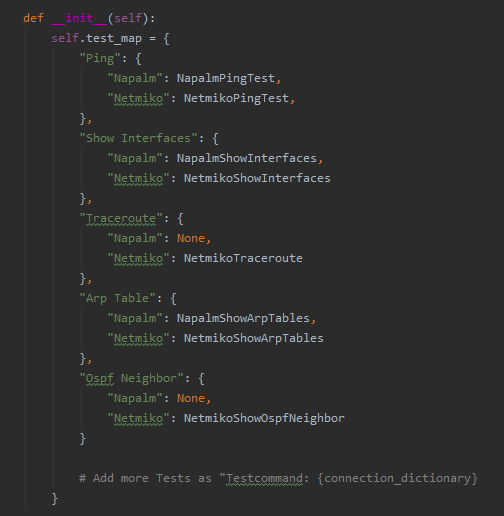
\includegraphics[scale=1.0]{\vorlagenOrdner/Bilder/Manual/strategyfactory.png}




\end{document}